\section{Absorbing Markov Chain Puzzles}

\begin{puzzle}
    Given the following absorbing Markov chain.
    \[
        T = \begin{bmatrix}
            1  & 0  & 0  & 0  \\
            .1 & .4 & .2 & .3 \\
            0  & 0  & 1  & 0  \\
            .4 & 0  & .2 & .4
        \end{bmatrix}
    \]
    \begin{enumerate}
        \item Identify the absorbing states.
        \item Write the solution matrix.
        \item Starting from state 4, what is the probability of eventual absorption in state 1?
        \item Starting from state 2, what is the probability of eventual absorption in state 3?
    \end{enumerate}
\end{puzzle}

\begin{puzzle}\label{puzzle_absorbing_markov_tennis}
    Two tennis players, Andre and Vijay each with two dollars in their pocket, decide to bet each other \$1, for every game they play. They continue playing until one of them is broke.
    \begin{enumerate}
        \item Write the transition matrix for Andre.
        \item Identify the absorbing states.
        \item Write the solution matrix.
        \item At a given stage if Andre has \$1, what is the chance that he will eventually lose it all?
    \end{enumerate}
\end{puzzle}


\begin{puzzle}
    Repeat Puzzle \ref{puzzle_absorbing_markov_tennis}, if the chance of winning for Andre is .4 and for Vijay .6.
    \begin{enumerate}
        \item Write the transition matrix for Andre.
        \item Write the solution matrix.
        \item If Andre has \$3, what is the probability that he will eventually be ruined?
        \item If Vijay has \$1, what is the probability that he will eventually triumph?
    \end{enumerate}
\end{puzzle}

\begin{puzzle}
    Repeat Puzzle \ref{puzzle_absorbing_markov_tennis}, if initially Andre has \$3 and Vijay has \$2.
    \begin{enumerate}
        \item Write the transition matrix.
        \item Identify the absorbing states.
        \item Write the solution matrix.
        \item If Andre has \$4, what is the probability that he will eventually be ruined?
    \end{enumerate}
\end{puzzle}

\begin{puzzle}
    The non-tenured professors at a community college are regularly evaluated. After an evaluation they are classified as good, bad, or improvable. The "improvable" are given a set of recommendations and are re-evaluated the following semester. At the next evaluation, 60\% of the improvable turn out to be good, 20\% bad, and 20\% improvable. These percentages never change and the process continues.
    \begin{enumerate}
        \item Write the transition matrix.
        \item Identify the absorbing states.
        \item Write the solution matrix.
        \item What is the probability that a professor who is improvable will eventually become good?
    \end{enumerate}
\end{puzzle}

\begin{puzzle}\label{puzzle_rat_maze}
    A rat is placed in the maze shown below, and it moves from room to room randomly. From any
    room, the rat will choose a door to the next room with equal probabilities. Once it reaches room
    1, it finds food and never leaves that room. And when it reaches room 5, it is trapped and cannot
    leave that room. What is the probability the rat will end up in room 5 if it was initially placed in
    room 3?

    % TODO Better version of this
    \begin{center}
        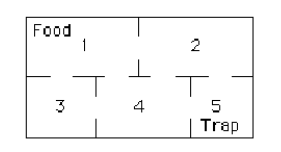
\includegraphics{chapters/markov_hw/section03/maze.png}
    \end{center}

    % \begin{tikzpicture}
    %     % Drawing the boxes
    %     \draw (0,0) rectangle (3,1);
    %     \draw (1,0) -- (1,1);
    %     \draw (2,0) -- (2,1);

    %     % Adding numbers
    %     \node at (0.5,0.5) {1};
    %     \node at (1.5,0.5) {2};
    %     \node at (2.5,0.5) {5};

    %     % Drawing lower boxes
    %     \draw (0,-1) rectangle (1,0);
    %     \draw (1,-1) rectangle (2,0);
    %     \node at (0.5,-0.5) {3};
    %     \node at (1.5,-0.5) {4};

    %     % Adding labels
    %     \node[above] at (0.5,1) {Food};
    %     \node[above] at (2.5,1) {Trap};
    % \end{tikzpicture}
\end{puzzle}

\begin{puzzle}
    In Puzzle \ref{puzzle_rat_maze}, what is the probability the rat will end up in room 1 if it was initially placed in
    room 2?

\end{puzzle}